\documentclass[12pt,a4paper]{article}
\usepackage[T2A]{fontenc}
\usepackage[utf8]{inputenc}
\usepackage[russian]{babel}
\usepackage{amsmath}
\usepackage{amssymb}
\usepackage{graphicx}
\usepackage{floatrow}
\usepackage{booktabs}
\usepackage{wrapfig}
\usepackage{lipsum}
\usepackage{subcaption}
\usepackage{fancyhdr}

\newcommand{\figref}[1]{(См. рис. \ref{#1})}
\newcommand{\secref}[1]{(См. раздел. \ref{#1})}

\newcommand{\e}[1]{\text{$\cdot10^{#1}$}}

\pagestyle{fancy}
\fancyhead{}
\fancyhead[L]{Работа 3.3.4}
\fancyhead[R]{}
\fancyfoot[C]{\thepage}

\author{\normalsize Выполнил: Голубович Тимур, группа Б01-108 \\
	\normalsize 08.10.2022}
\date{}

\usepackage{float}
\restylefloat{table}
\title
{
	\large Отчет о выполнении лабораторной работы 3.3.4 \\
	\Large Эффект Холла в полупроводниках \\ 
}


\begin{document}
\maketitle
	
\section*{Цель работы}
Измерение подвижности и концентрации носителей заряда в полупроводниках.

\section*{Оборудование и приборы} 
Электромагнит с регулируемым источником питания $GPR$; \newline
батарейка 1,5 В; \newline
амперметр; \newline
реостат; \newline
цифровой вольтметр B7-78/1; \newline
милливеберметр M119; \newline
образцы легированного германия. \newline
	

\section*{Теоретическое введение}

В электрическом поле $\vec{E}$ на заряды действует сила $q\vec{E}$. Во внешнем магнитном поле $\vec{B}$ на движущиеся заряды также действует сила Лоренца:

$$ \vec{F} = q\vec{E} + q\vec{u} \times \vec{B}.$$

Эта сила вызывает движение носителей, направление которого в общем случае не совпадает с $\vec{E}$. Действительно, траектории частиц будут либо искривляться, либо, если геометрия проводника этого не позволяет, возникнет дополнительное электрическое поле, компенсирующее магнитную составляющую силы Лоренца. Возникновение поперечного току электрического поля в образце, помещённом во внешнее магнитное поле, называют эффектом Холла.


\begin{figure}[h]
	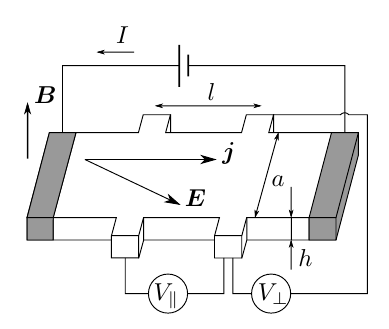
\includegraphics[width = 7 cm]{res/scheme_hall.png}
	\caption{Схема мостика Холла}
	\label{fig:scheme_hall}
\end{figure}

В данной работе для проверки эффекта Холла будем использовать мостик Холла \ref{fig:scheme_hall}.

Для поперечного (холловского) напряжения получаем:

$$ U_\perp = E_y a = \rho_{yx} \cdot j_x a= \frac{j_x B}{n q}. $$
Учитывая, что $j_x = \frac{I}{ah}$, получаем:

\begin{equation}
	\label{U_perp}
	U_\perp = \frac{B}{nqh} \cdot I = R_H \cdot \frac{B}{h} \cdot I,
\end{equation}
где $R_H = \frac{1}{nq}$ -- постоянная Холла.

Для продольной составляющей напряжения:

$$ U_\parallel = E_x l = j_x / \sigma_0 l = I R_0, $$
где $R_0 = \frac{l}{\sigma_0 a h}$.

\begin{equation}
	\label{sigma_0}
	\sigma_0 = \frac{I \cdot l}{U_{35} \cdot h \cdot a}.
\end{equation}


\section*{Экспериментальная установка}

Установка, используемая в работе, представлена на рис. \ref{fig:scheme}.

\begin{figure}[H]
    \centering
	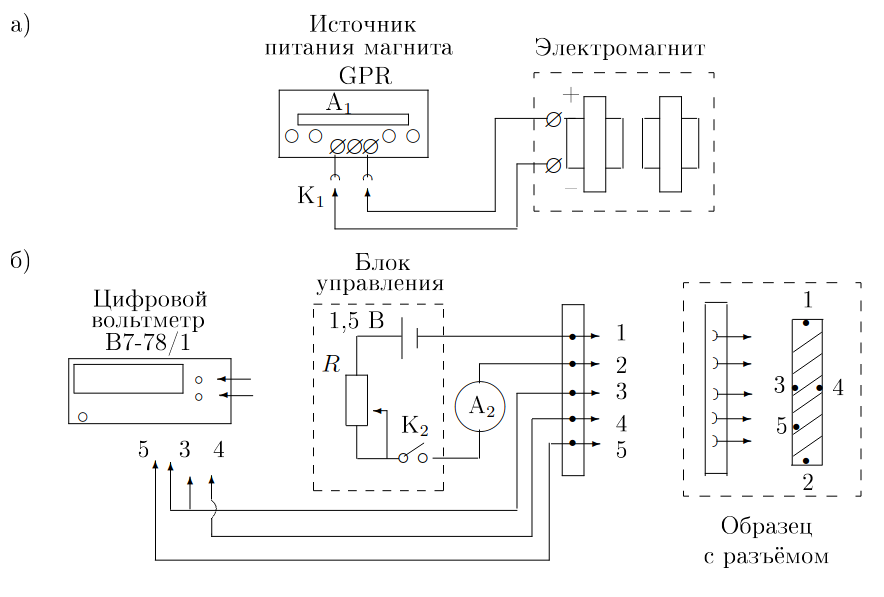
\includegraphics[width = 10 cm]{res/scheme.png}
	\caption{Схема установки для исследования эффекта Холла в полупроводниках}
	\label{fig:scheme}
\end{figure}

В зазоре электромагнита \ref{fig:scheme} создаётся постоянное магнитное поле, величину которого можно менять с помощью регулятора источника питания электромагнита. Ток питания электромагнита измеряется амперметром $A_1$.

Градуировка электромагнита проводится при помощи милливеберметра и миллитесламетра.

Прямоугольный образец из легированного германия, смонтированный в специальном держателе \ref{fig:scheme}, подключается к источнику питания ($\approx$ 1,5 В). При замыкании ключа $K_2$ вдоль длинной стороны образца (контакты 3, 5) течёт ток, величина которого регулируется реостатом $R_2$ и измеряется миллиамперметром $A_2$.

В образце с током, помещенном в зазор электромагнита, между контактами 3 и 4 возникает разность потенциалов $U_{34}$, которая измеряется с помощью цифрового вольтметра.

Контакты 3 и 4 вследствие неточности подпайки могут не лежать на эквипотенциали, для устранения этого эффекта будем измерять начальное значение напряжения $U_0$ (при выключенном магните) в каждой серии измерений.




\section*{Ход работы}
	
	\subsection*{Градуировка электромагнита}
	
	Занесём все параметры установки в таблицу \ref{tab:def}.
	
	\begin{table}[H]
	    \caption{Результаты измерений индукции магнита}
		\begin{tabular}{ccccc}
\toprule
$S\cdot N, \text{см}^2\cdot\text{вит}$ & $r_\text{внеш}, \text{Ом}$ &  $a, \text{мм}$ &  $L_{3,5}, \text{мм}$ &  $l, \text{мм}$ \\
\midrule
72 & $<=5$ & 1,5 & 3,0 & 1,7 \\
\bottomrule
\end{tabular}
		\label{tab:def}
	\end{table}
	
	Проведем градуировку электромагнита. Для этого измерим зависимость $B(I)$, где $B$ -- модуль вектора индукции магнитного поле в зазоре, $I_M$ -- ток, протекающий через обмотки магнита. Измерения проведем милливеберметром. Погрешности данных приборов:
	
	$$ \varsigma_{\text{Вб}} = 0.15$$
	
	Точность измерения $I_M$ определяется точностью амперметра, встроенного в лабораторный блок питания GPR: $$\varsigma_{A_1} = 0.005 \; \text{А}$$
	
	\begin{table}[H]
		\begin{tabular}{ccccc}
\toprule
$I_M, \text{A}$ & $\Phi_\text{н}, \text{мВб}$ &  $\Phi_\text{к}, \text{мВб}$ &  $\Phi, \text{мВб}$ &  $B, \text{Тл}$ \\
\midrule
0,00 & 0,2 & 0,4 & 0,2 & 0,028 \\
0,25 & 0,1 & 1,7 & 1,6 & 0,222 \\
0,50 & 0,1 & 3,1 & 3,0 & 0,417 \\
0,75 & 0,2 & 4,5 & 4,3 & 0,597 \\
1,00 & 0,1 & 5,6 & 5,5 & 0,764 \\
1,25 & 0,1 & 6,7 & 6,6 & 0,917 \\
1,50 & 0,2 & 7,5 & 7,3 & 1,014 \\
1,75 & 0,1 & 7,9 & 7,8 & 1,083 \\
2,00 & 0,1 & 8,3 & 8,2 & 1,139 \\
\bottomrule
\end{tabular}

		\caption{Результаты измерений индукции магнита}
		\label{tab:ind}
	\end{table}

	Построим графики $B(I)$ по результатам измерения магнитного поля милливеберметром.
	
	\begin{figure}[H]
		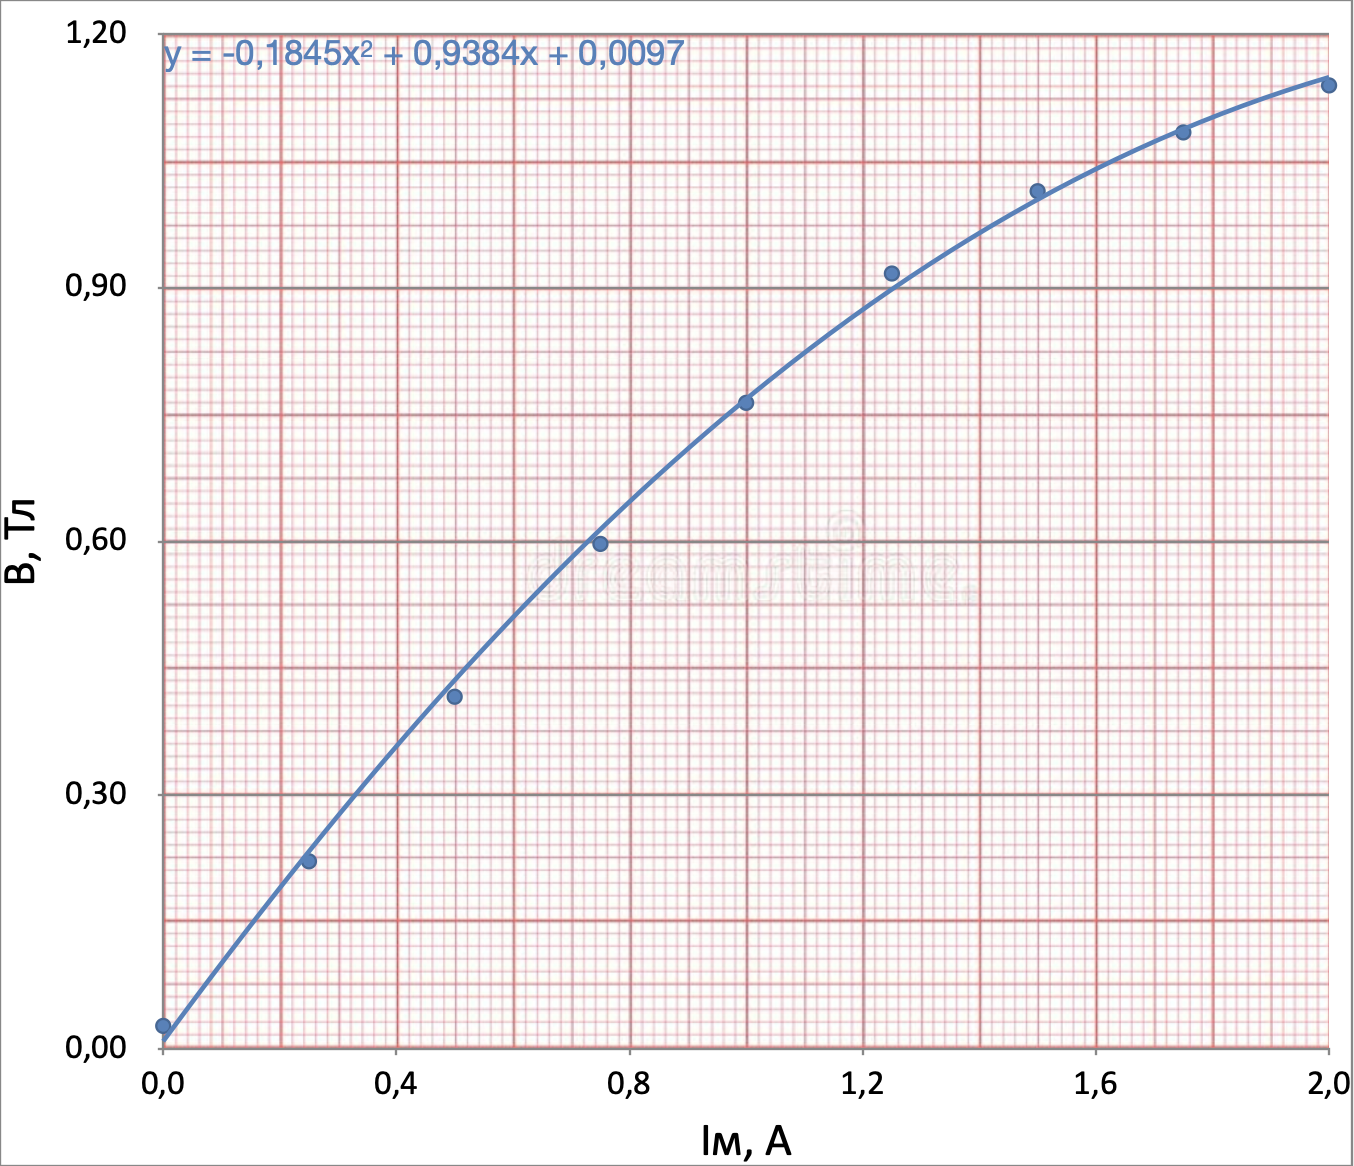
\includegraphics[width = 10 cm]{src/electromagnet_BI.png}
		\caption{$B(I_M)$}
	\end{figure}

	Как видно из графика, зависимость индукции от тока в обмотке нелинейная. Поэтому для дальнейших расчётов интерполируем ее полиномом второй степени.
	
	\subsection*{ЭДС Холла}

	Проведем измерения $U_{34}(I_M)$ для различных $I$. Рассчитаем значения $B$ и занесем в таблицу.
	Измерения $I$ делаются миллиамперметром с $\varsigma_{A_2} = 5 \; \text{мкА} $.
	Измерения $U$ проводятся вольтметром $V_1$, модель B7-78/1: $\varsigma_{V_1} = 3.5 \; \text{мкВ}$.
	В измерениях учитывается $U_0$ -- сдвиг напряжения при нулевом магнитном поле, возникающий из-за неточности подпайки.
	
	\begin{table}[H]
		\addtolength{\tabcolsep}{-4pt}
		\footnotesize
		\begin{tabular}{cccc|cccc}
\toprule
$U$, мВ & $I_\text{м}$, А & $B$, Тл & $I\cdot B$, мА$\cdot$Тл &
$U$, мВ & $I_\text{м}$, А & $B$, Тл & $I\cdot B$, мА$\cdot$Тл \\

\multicolumn{4}{c}{$I$ = 0,3 мА} & \multicolumn{4}{c}{$I$ = 0,4 мА} \\

-0,017 & 0,00 & 0,01 & 0,003 & -0,023 & 0,00 & 0,01 & 0,004 \\
 0,004 & 0,25 & 0,23 & 0,070 &  0,005 & 0,25 & 0,23 & 0,093 \\
 0,026 & 0,50 & 0,43 & 0,130 &  0,036 & 0,50 & 0,43 & 0,173 \\
 0,049 & 0,75 & 0,61 & 0,183 &  0,060 & 0,75 & 0,61 & 0,244 \\
 0,067 & 1,00 & 0,76 & 0,229 &  0,091 & 1,00 & 0,76 & 0,305 \\
 0,083 & 1,25 & 0,89 & 0,268 &  0,114 & 1,25 & 0,89 & 0,358 \\
 0,095 & 1,50 & 1,00 & 0,301 &  0,130 & 1,50 & 1,00 & 0,401 \\
 0,104 & 1,75 & 1,09 & 0,326 &  0,140 & 1,75 & 1,09 & 0,435 \\
 0,110 & 2,00 & 1,15 & 0,345 &  0,148 & 2,00 & 1,15 & 0,459 \\
 0,112 & 2,08 & 1,16 & 0,349 &  0,150 & 2,06 & 1,16 & 0,464 \\

 \multicolumn{4}{c}{$I$ = 0,5 мА} & \multicolumn{4}{c}{$I$ = 0,6 мА}\\
 
 -0,028 & 0,00 & 0,01 & 0,005 & -0,035 & 0,00 & 0,01 & 0,006 \\
 0,006 & 0,25 & 0,23 & 0,116 &  0,010 & 0,25 & 0,23 & 0,140 \\
 0,045 & 0,50 & 0,43 & 0,216 &  0,055 & 0,50 & 0,43 & 0,260 \\
 0,080 & 0,75 & 0,61 & 0,305 &  0,097 & 0,75 & 0,61 & 0,366 \\
 0,113 & 1,00 & 0,76 & 0,382 &  0,136 & 1,00 & 0,76 & 0,458 \\
 0,140 & 1,25 & 0,89 & 0,447 &  0,170 & 1,25 & 0,89 & 0,537 \\
 0,160 & 1,50 & 1,00 & 0,501 &  0,194 & 1,50 & 1,00 & 0,601 \\
 0,173 & 1,75 & 1,09 & 0,543 &  0,210 & 1,75 & 1,09 & 0,652 \\
 0,184 & 2,00 & 1,15 & 0,574 &  0,223 & 2,00 & 1,15 & 0,689 \\
 0,186 & 2,06 & 1,16 & 0,580 &  0,225 & 2,05 & 1,16 & 0,695 \\
 
  \multicolumn{4}{c}{$I$ = 0,7 мА} & \multicolumn{4}{c}{$I$ = 0,8 мА}\\
  
 -0,040	&0,00	&0,01	&0,007	&0,047	&0,00	&0,01	&0,008	\\
 0,010	&0,25	&0,23	&0,163	&0,010	&0,25	&0,23	&0,186	\\
 0,063	&0,50	&0,43	&0,303	&0,072	&0,50	&0,43	&0,346	\\
 0,115	&0,75	&0,61	&0,427	&0,133	&0,75	&0,61	&0,488	\\
 0,159	&1,00	&0,76	&0,535	&0,183	&1,00	&0,76	&0,611	\\
 0,197	&1,25	&0,89	&0,626	&0,228	&1,25	&0,89	&0,716	\\
 0,226	&1,50	&1,00	&0,702	&0,258	&1,50	&1,00	&0,802	\\
 0,246	&1,75	&1,09	&0,761	&0,281	&1,75	&1,09	&0,869	\\
 0,260	&2,00	&1,15	&0,804	&0,297	&2,00	&1,15	&0,919	\\
 0,262	&2,04	&1,16	&0,809	&0,298	&2,02	&1,15	&0,922	\\
 
 \multicolumn{4}{c}{$I$ = 0,9 мА} & \multicolumn{4}{c}{$I$ = 1,0 мА}\\
 
 -0,053 &0,00	&0,01	&0,009	&-0,059 &0,00 &0,01 &0,010\\
 0,012 &0,25	&0,23	&0,209	& 0,016 &0,25 &0,23 &0,233\\
 0,080 &0,50	&0,43	&0,389	& 0,091 &0,50 &0,43 &0,433\\
 0,147 &0,75	&0,61	&0,549	& 0,164 &0,75 &0,61 &0,610\\
 0,205 &1,00	&0,76	&0,687	& 0,230 &1,00 &0,76 &0,764\\
 0,255 &1,25	&0,89	&0,805	& 0,283 &1,25 &0,89 &0,894\\
 0,291 &1,50	&1,00	&0,902	& 0,324 &1,50 &1,00 &1,002\\
 0,316 &1,75	&1,09	&0,978	& 0,352 &1,75 &1,09 &1,087\\
 0,334 &2,00	&1,15	&1,034	& 0,374 &2,00 &1,15 &1,149\\
 0,335 &2,01	&1,15	&1,035	&       &     &     &     \\
 
\bottomrule
\end{tabular}

		\caption{Результаты измерений $U_{34}(I_M)$ и обработки $B$ и $B\cdot I$}
	\end{table}

	По методу наименьших квадратов рассчитаем параметры графиков, считая зависимость линейной. В результате получим значение углового коэффициента $K = \frac{\Delta \mathcal{E}_H}{\Delta B}$ для каждого графика. Построим график $K(I)$ и рассчитаем его параметры.
	
	\begin{figure}[H]
		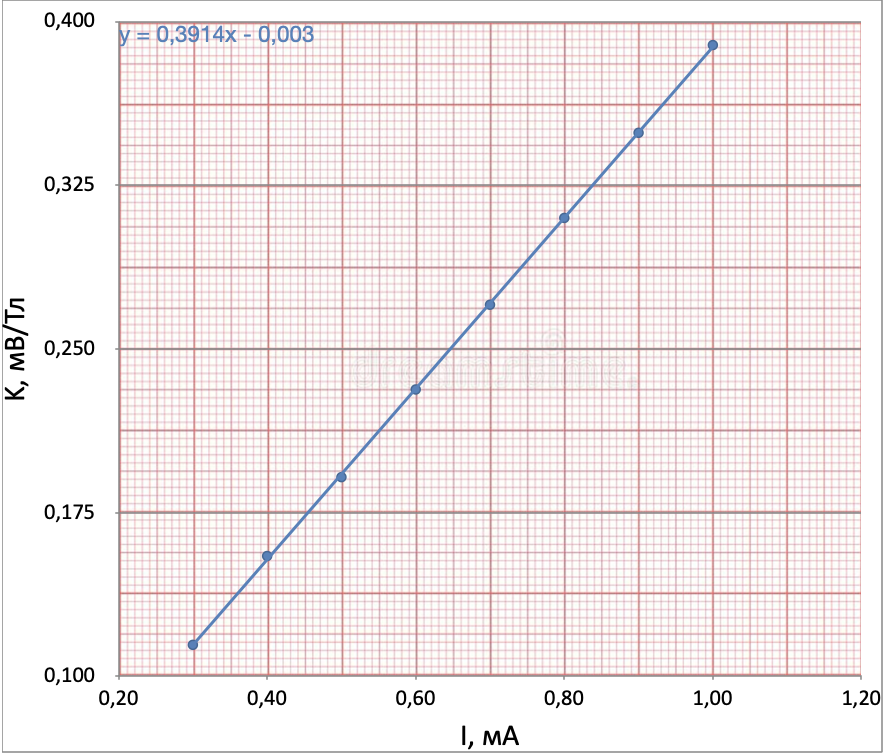
\includegraphics[width = 10 cm]{src/hallEMF_KI.png}
		\caption{График зависимости углового коэффициента от тока через образец}
	\end{figure}
	
	\begin{table}[h]
		\begin{tabular}{cc}
\toprule
$I$, мА & $K$, $\frac{\text{мВ}}{\text{Тл}}$ \\
\midrule
0,3 & 0,114 \\
0,4 & 0,155 \\
0,5 & 0,191 \\
0,6 & 0,231 \\
0,7 & 0,270 \\
0,8 & 0,310 \\
0,9 & 0,349 \\
1,0 & 0,389 \\
\bottomrule
\end{tabular}

		\caption{Зависимость углового коэффициента от тока через образец}
	\end{table}
	
	\begin{table}[h]
		\caption{Параметры графика $K(I)$}
		\begin{tabular}{l|cccc}
	\toprule
	& $a$, $\frac{\text{Ом}}{\text{Тл}}$ & $\varepsilon_a$, \% & $b$, $\frac{\text{мВ}}{\text{Тл}}$ & $\varepsilon_b$, \% \\ \midrule
	$K=a\cdot I + b$ & 0,391 & 0,8 & -0,003 & 70 \\
\bottomrule
\end{tabular}
	\end{table}

	Выясним знак носителей заряда в легированном германии. Мы знаем, что электрическое поле направлено от $4$ к $3,5$ из знака напряжения на вольтметре $V1$. Воспользовавшись правилом буравчика и правилом левой руки получим, что сила Лоренца направлена от $3,5$ к $4$ для обоих знаков зарядов. Следовательно, носитель заряда в легированном германии имеет положительный заряд (электронная проводимость).
	
	\begin{figure}[H]
		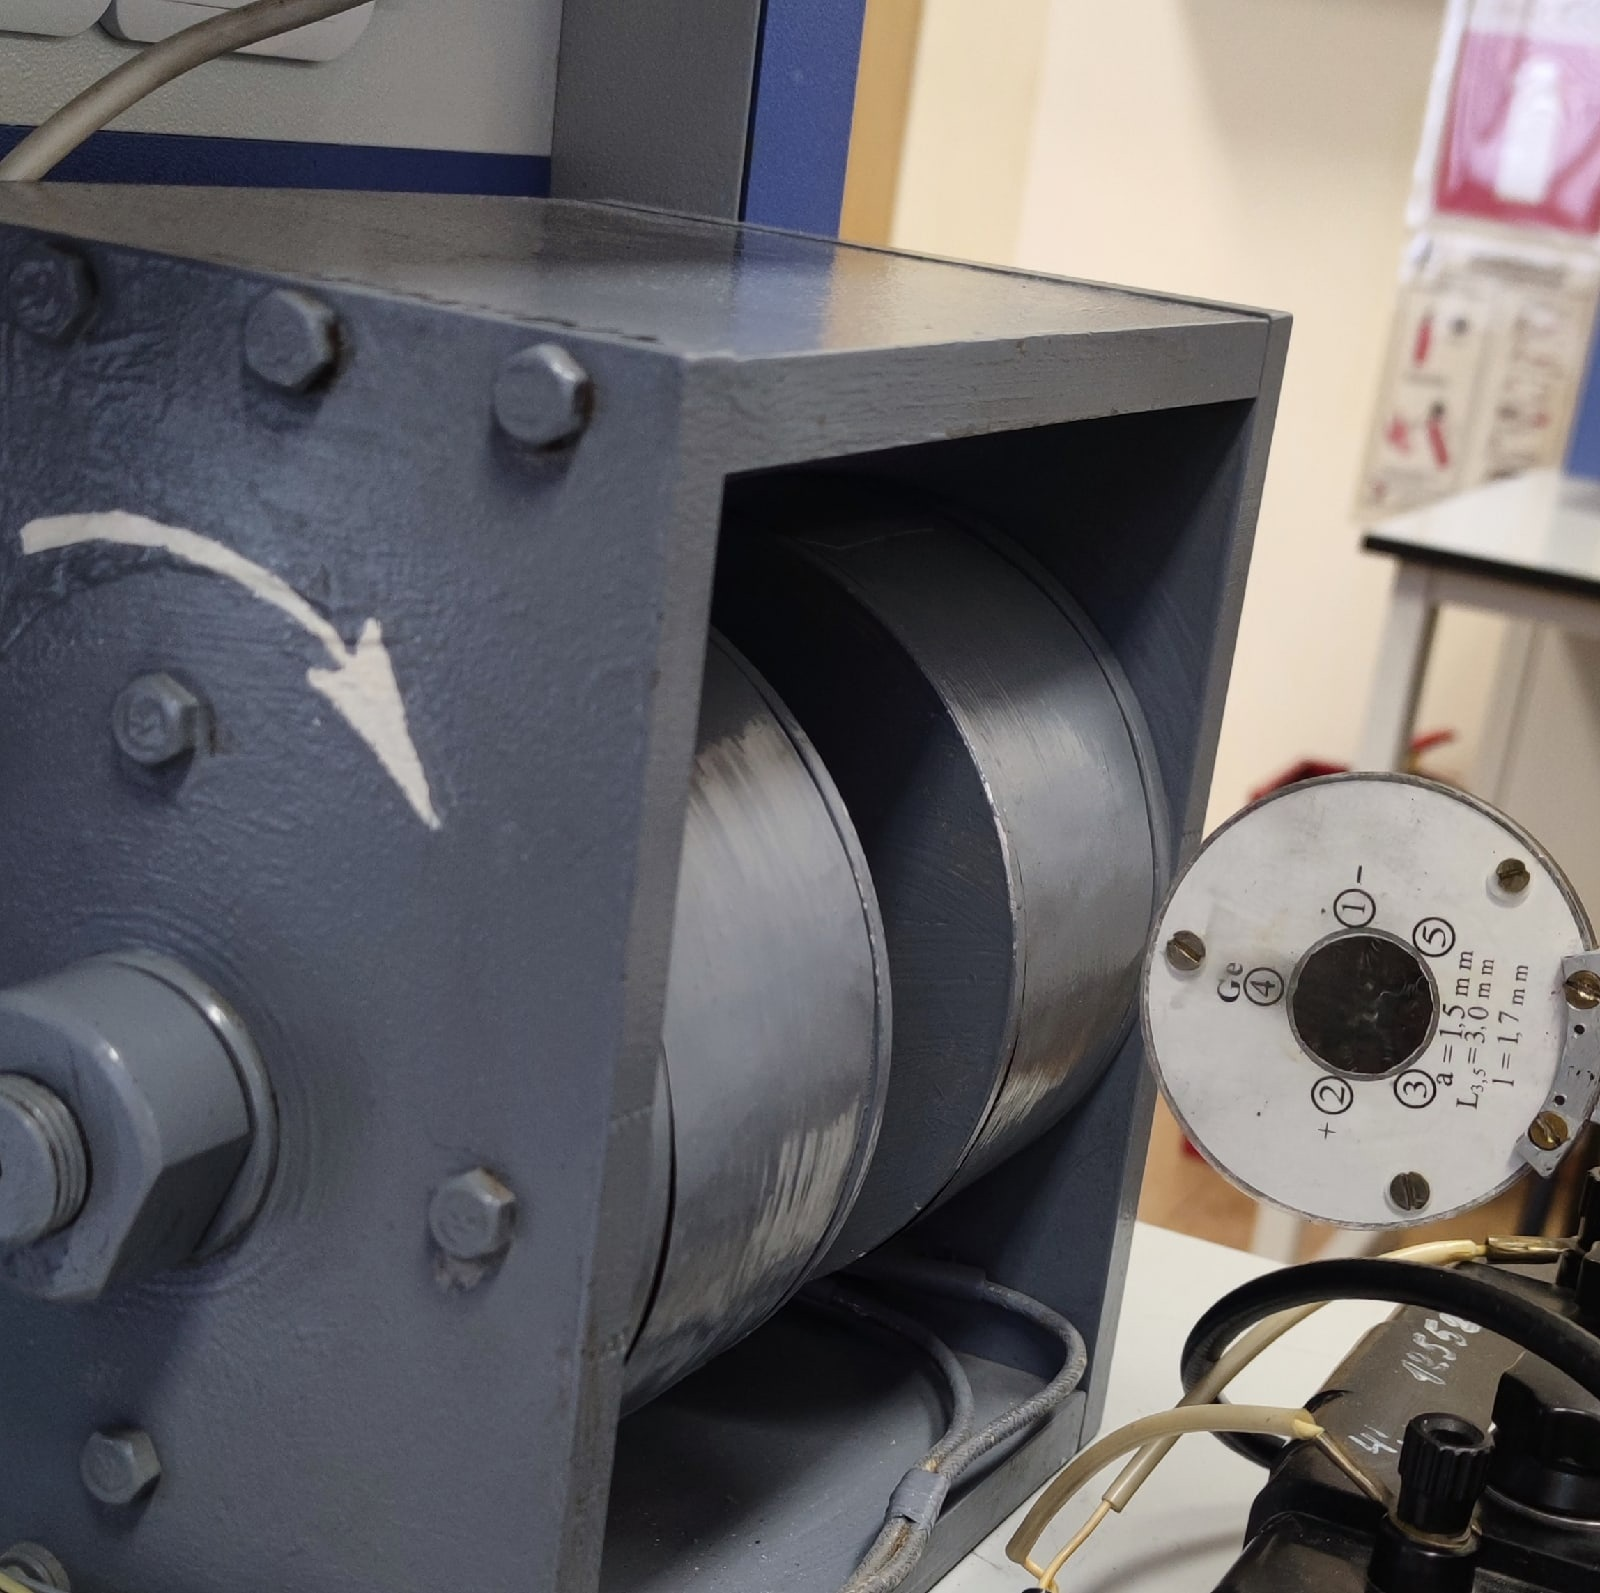
\includegraphics[width = 10 cm]{res/probe_coil.jpeg}
		\caption{Пробная катушка и ее положение относительно магнита}
	\end{figure}
	
	Определим коэффициент Холла $R_H$ по формуле \eqref{U_perp}:
	$$ R_H = h \frac{U_\perp}{BI} = h \cdot a_K = 1.5 \; \text{мм} \cdot 0,391 \; \frac{\text{В}}{\text{Тл} \cdot \text{А}} = (5.87 \pm 0.4) \cdot 10^{-4} \; \frac{\text{м}^3}{\text{Кл}} $$
	
	Определим концентрацию $n$:
	$$ n = \frac{1}{R_H e} = (1.06 \pm 0.4) \cdot 10^{22} \frac{1}{\text{м}^3} $$
	
	\subsubsection*{Альтернативный метод обработки}
	
	Также для определения искомого параметра можно воспользоваться тем, что:
	$$ \mathcal{E}_H = \frac{R_H}{h} \cdot BI $$
	
	Построим график $\mathcal{E}_H (BI)$ и определим его параметры.
	
	\begin{figure}[H]
		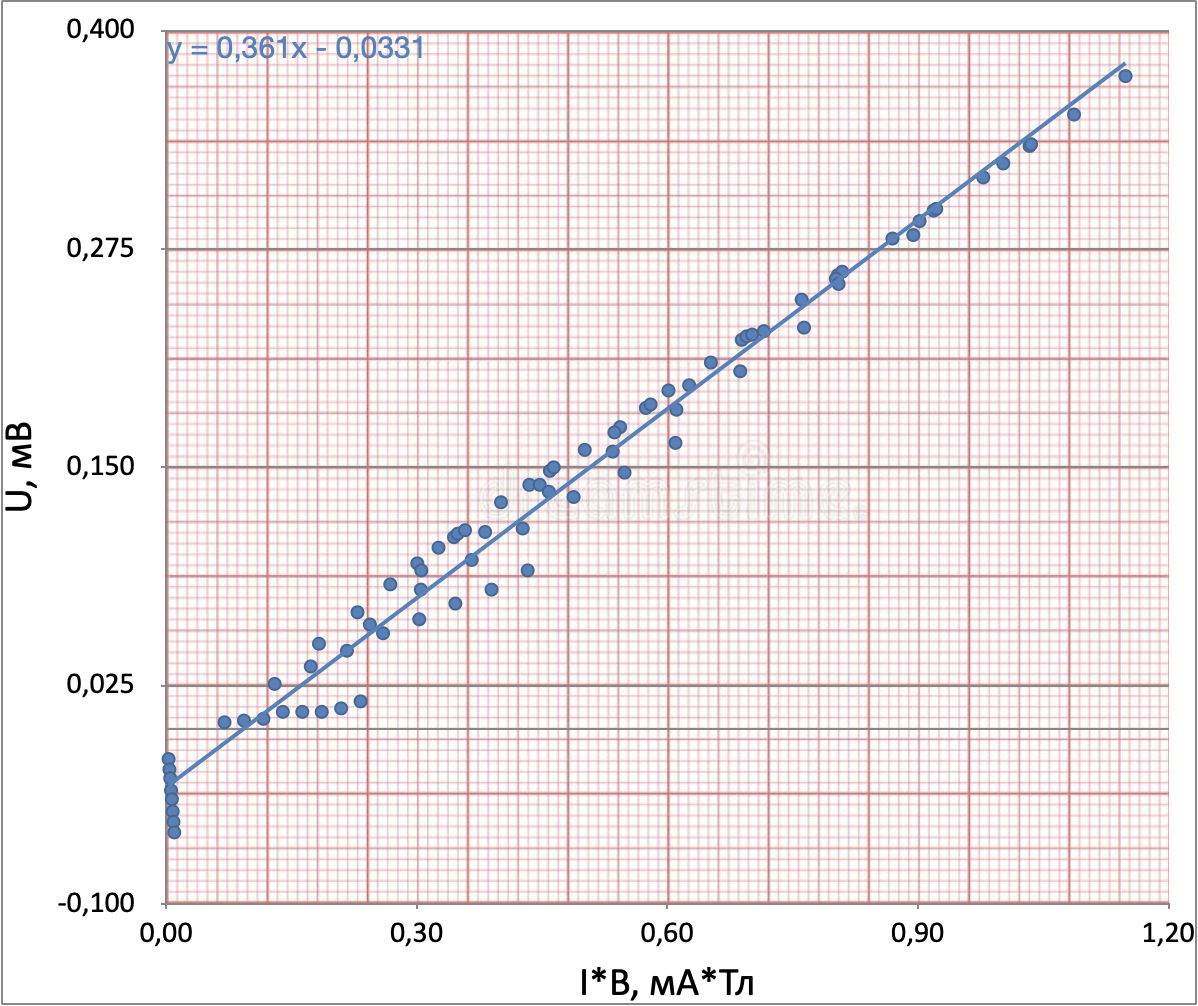
\includegraphics[width = 10 cm]{src/hallEMF_UIB.png}
		\caption{Зависимость холловского напряжения от произведения индукции поля и тока в образце}
	\end{figure}
	
	\begin{table}[h]
		\caption{Параметры графика $\mathcal{E}_H (IB)$}
		\begin{tabular}{l|cccc}
	\toprule
	 & $a$, $\frac{\text{Ом}}{\text{Тл}}$ & $\varepsilon_a$, \% & $b$, $\frac{\text{мВ}}{\text{Тл}}$ & $\varepsilon_b$, \% \\ \midrule
	$U=a\cdot IB + b$ & 0,382 & 0,8 & -0,021 & 3 \\
\bottomrule
\end{tabular}

	\end{table}

	Определим коэффициент Холла $R_H$ по формуле \eqref{U_perp}:
	$$ R_H = h \frac{U_\perp}{BI} = h \cdot a_{IB} = 1.5 \; \text{мм} \cdot 0.382 \; \frac{\text{В}}{\text{Тл} \cdot \text{А}} = (5.73 \pm 0.4) \cdot 10^{-4} \; \frac{\text{м}^3}{\text{Кл}} $$
	
	Определим концентрацию $n$:
	$$ n = \frac{1}{R_H e} = (1.09 \pm 0.5) \cdot 10^{22} \frac{1}{\text{м}^3} $$
	
	\subsection*{Удельная проводимость}
	
	Измерим $U_{35} (I)$ в образце. Построим график $U_{35} (I)$ и рассчитаем его параметры.
	
	\begin{table}[h]
		\caption{Результаты измерений $I(U_{35})$}
		\begin{tabular}{cc}
\toprule
$I$, мА & $U_{35}$, мВ \\
\midrule
0,3 & 0,114 \\
0,4 & 0,155 \\
0,5 & 0,191 \\
0,6 & 0,231 \\
0,7 & 0,270 \\
0,8 & 0,310 \\
0,9 & 0,349 \\
1,0 & 0,389 \\
\bottomrule
\end{tabular}

	\end{table}
	
	\begin{figure}[H]
		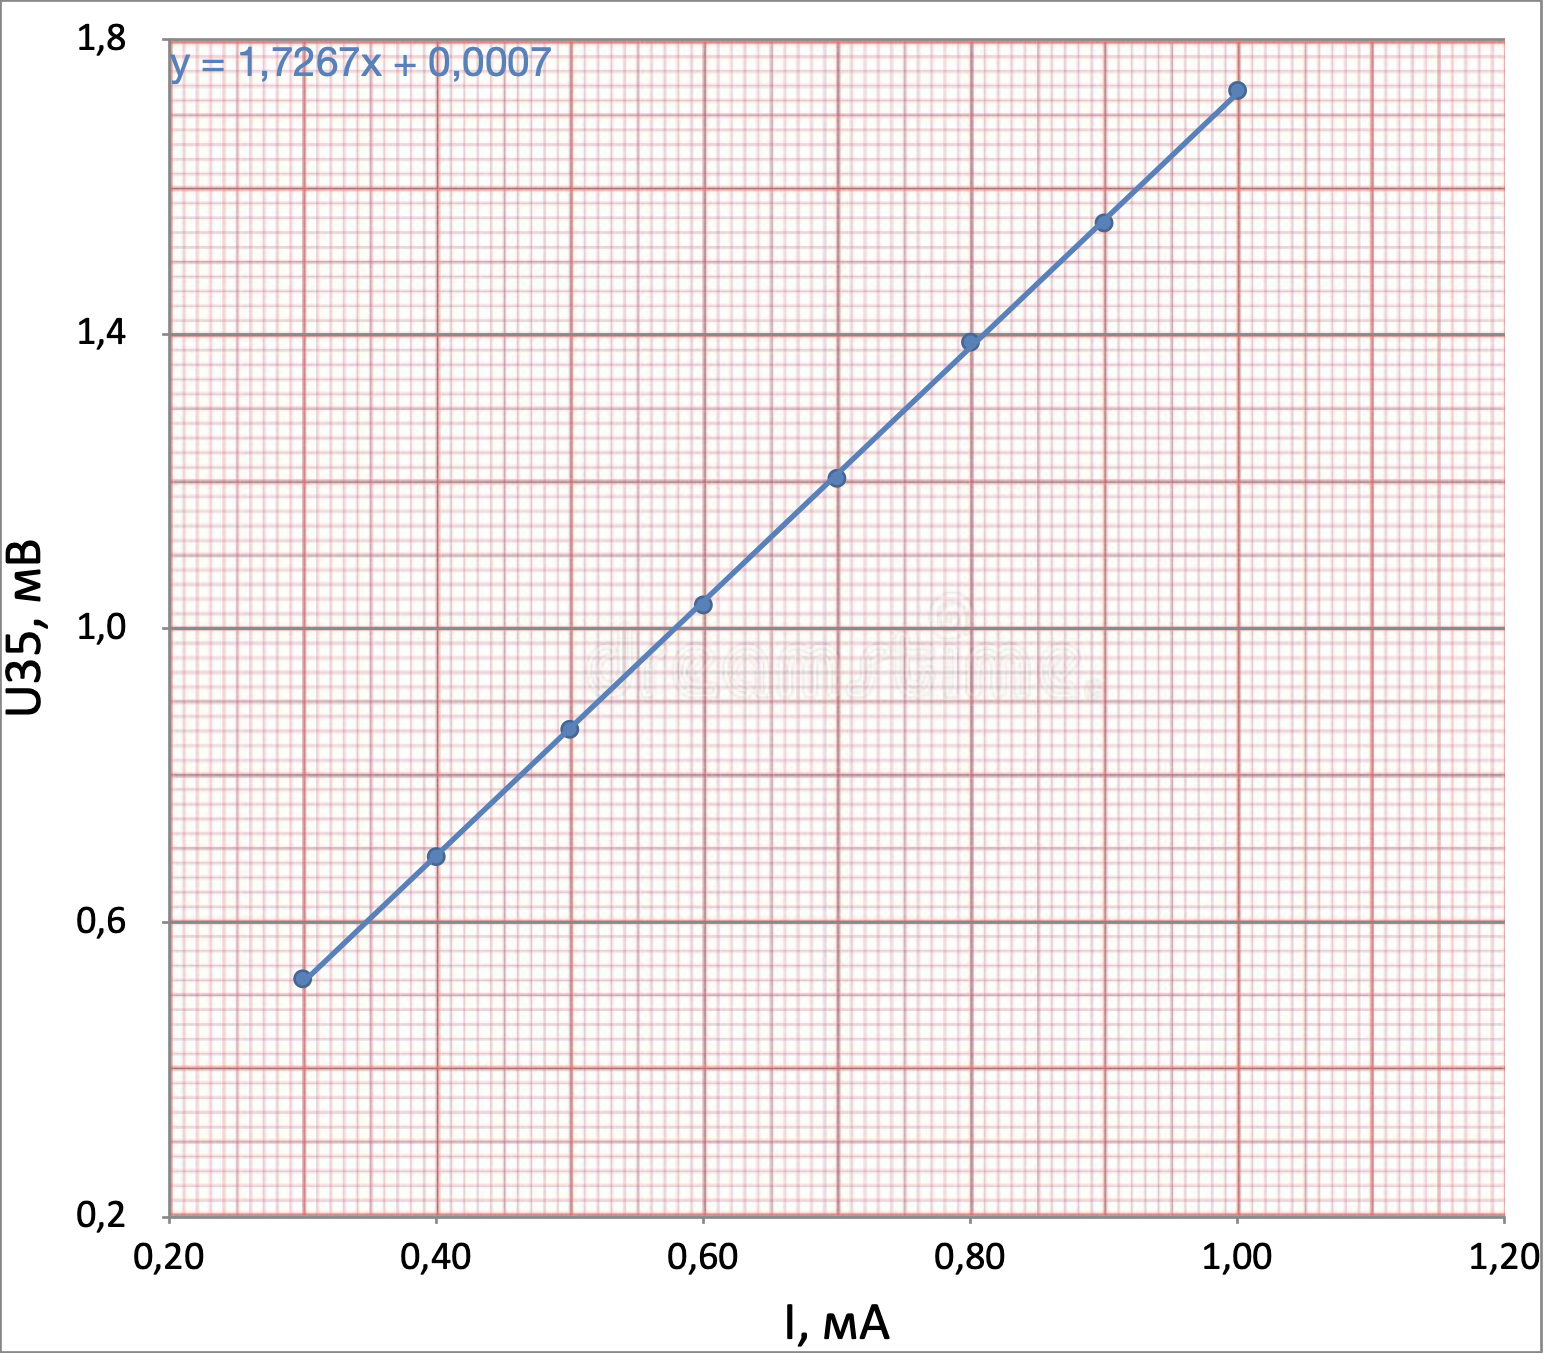
\includegraphics[width = 10 cm]{src/cond_UI.png}
		\caption{Зависимость напряжения $U_{35}$ от основного тока в образце}
	\end{figure}
	
	\begin{table}[h]
		\caption{Параметры графика $U_{35} (I)$}
		\begin{tabular}{l|cccc}
	\toprule
	 & $a$, Ом & $\varepsilon_a$, \% & $b$, мВ & $\varepsilon_b$, \% \\ \midrule
	$U=a\cdot I + b$ & 1,727 & 0,9 & 0,001 & 1600 \\
\bottomrule
\end{tabular}
	\end{table}
	
	Рассчитаем удельную проводимость $\sigma_0$:
	$$ \sigma_0 = \frac{I \cdot l}{U_{35} \cdot h \cdot a} = \frac{ 3.0 \; \text{мм} }{ 1.73 \; \text{Ом} \cdot 1.5 \; \text{мм} \cdot 1.7 \; \text{мм}} = (681 \pm 51) \frac{1}{\text{Ом} \cdot \text{м}} $$
	
	Рассчитаем подвижность зарядов $b$:
	$$ b = \frac{\sigma_0}{e n} = (4015 \pm 420) \frac{\text{см}^2}{\text{В} \cdot \text{с}} $$


\section*{Вывод}

	Данная работа подтверждает существование эффекта Холла в полупроводниках.
	
	Получено значение коэффициента Холла $ R_H = (5.7 \pm 0.4) \cdot 10^{-4} \; \frac{\text{м}^3}{\text{Кл}} $. Также в работе оценено значение концентрации носителей тока в образце $ n = (1.06 \pm 0.4) \cdot 10^{22} \; \frac{1}{\text{м}^3} $, удельная проводимость $ \sigma_0 = (681 \pm 51) \; \frac{1}{\text{Ом} \cdot \text{м}} $, подвижность носителей $ b = \frac{\sigma_0}{e n} = (4015 \pm 420) \; \frac{\text{см}^2}{\text{В} \cdot \text{с}} $.
	
	Справочные данные для данного образца германия отсутствуют, большинство параметров зависят от степени легирования. Значения подвижности носителей зависит от легирующего элемента и лежат в пределах $(2000 \div 3000) \; \frac{\text{см}^2}{\text{В} \cdot \text{с}}$.
	

	
\begin{thebibliography}{9}
	\bibitem{max} \emph{Лабораторный практикум по общей физике. В 3 томах. Том 2. Электричество и магнетизм: учебное пособие} под ред. А. В. Максимычева, М. Г. Никулина
	\bibitem{max} \emph{Эффект Холла в германии, легированном разными примесями} Г. П. Гайдар, Е. Ю. Гайворонская, 2017
\end{thebibliography}
\end{document}
